\documentclass[11pt]{article}
\usepackage[utf8]{inputenc}
\usepackage{amsmath,amssymb}
\usepackage{hyperref}
\usepackage[margin=1in]{geometry}
\usepackage{listings}
\usepackage{xcolor}
\usepackage{booktabs}
\usepackage{inconsolata}
\usepackage{graphicx}

\definecolor{codegreen}{rgb}{0,0.6,0}
\definecolor{codegray}{rgb}{0.5,0.5,0.5}
\definecolor{codepurple}{rgb}{0.58,0,0.82}
\definecolor{backcolour}{rgb}{0.95,0.95,0.92}

\lstset{
    backgroundcolor=\color{backcolour},
    commentstyle=\color{codegreen},
    keywordstyle=\color{blue},
    numberstyle=\tiny\color{codegray},
    stringstyle=\color{codepurple},
    basicstyle=\ttfamily\small,
    breakatwhitespace=false,
    breaklines=true,
    captionpos=b,
    keepspaces=true,
    numbers=left,
    numbersep=5pt,
    showspaces=false,
    showstringspaces=false,
    showtabs=false,
    tabsize=4,
    language=Python
}

\title{\textbf{Student's Companion Guide}\\[2pt]\large Exploring Riemann's Mathematics with Python}
\author{\textbf{Chaman Singh Verma}}
\date{July 19, 2026}

\begin{document}

\maketitle

Welcome! This guide is a student-friendly companion to the formal paper on Bernhard Riemann's mathematical discoveries.

While academic papers use advanced complex analysis and differential geometry, this guide is written to be accessible to advanced high-school and early undergraduate students. It explains the core concepts using high-school algebra, visual metaphors, and simple Python code, assuming only a brief exposure to complex numbers and basic trigonometry. By combining mathematics with programming, you can see these deep discoveries come to life on your own computer!

\section{Topic Roadmap}
The table below provides a quick reference to the topics covered in this guide, matching each mathematical concept with its Python implementation and real-world application.

\begin{table}[h!]
\centering
\small
\resizebox{\textwidth}{!}{%
\begin{tabular}{llll}
\toprule
\textbf{Topic} & \textbf{Core Math Concept} & \textbf{Python Function} & \textbf{Real-World Application} \\
\midrule
1. Zeta Function \& Hypothesis & Zeros on the complex critical line & \texttt{riemann\_zeta} & Prime distribution \& primality testing \\
2. Riemann Integration & Approximating integrals with sums & \texttt{riemann\_sum} & Numerical computing \& calculus \\
3. Prime Counting \& $\operatorname{Li}(x)$ & Gauss-Riemann prime approximations & \texttt{logarithmic\_integral\_li} & Computational number theory \\
4. Spherical Geodesics & Geodesic distances on curved spheres & \texttt{spherical\_distance} & GPS aviation mapping \& cosmology \\
5. General Riemannian Geometry & Metric tensor, curvature, geodesic ODEs & \texttt{christoffel\_symbols}, \texttt{riemann\_curvature\_tensor}, \texttt{solve\_geodesic} & General relativity, robotics, graphics \\
\bottomrule
\end{tabular}%
}
\caption{Roadmap of Riemann's concepts explored in this guide.}
\label{tab:roadmap}
\end{table}

\section{Getting Started: How to Run the Code}

All of the mathematical concepts discussed in this guide are implemented in the Python program \texttt{riemann\_codes.py}.

To run the interactive demonstration on your computer:
\begin{enumerate}
    \item Open your terminal (macOS/Linux) or Command Prompt (Windows).
    \item Navigate to the folder containing the project files.
    \item Execute the following command to run all six demos in sequence:
    \begin{lstlisting}[language=bash,numbers=none]
python3 riemann_codes.py
    \end{lstlisting}
    \item To call the demos individually from a Python interactive session, first import the module, then call any demo function:
    \begin{lstlisting}[language=bash,numbers=none]
python3
>>> from riemann_codes import demo_zeta_function, demo_riemann_integration, \
...     demo_prime_distribution, demo_riemannian_geometry, \
...     demo_general_riemannian_geometry, demo_explicit_formula
>>> demo_zeta_function()
    \end{lstlisting}
    \item \textbf{Visualizations:} If you have \texttt{matplotlib} and \texttt{numpy} installed (\texttt{pip install matplotlib numpy}), you can generate publication-quality plots:
    \begin{lstlisting}[language=bash,numbers=none]
python3 -c "from riemann_visualize import generate_all_plots; generate_all_plots('plots')"
    \end{lstlisting}
    This creates four PNG files in a \texttt{plots/} directory: zeta critical line, prime staircase, geodesics on manifolds, and sectional curvature.
\end{enumerate}
This will run the built-in simulations and print the results directly to your screen.

\section{The Riemann Zeta Function \& the Critical Line}

\subsection{Why Riemann Cared: The Prime Number Mystery}
In 1859, Riemann was 32 years old and had just been elected to the Berlin Academy. His memoir "On the Number of Primes Less Than a Given Magnitude" was only 8 pages long, but it changed mathematics forever. The problem: primes (2, 3, 5, 7, 11, 13...) look random, but Gauss and Legendre had conjectured they follow a smooth density $\pi(x) \sim x/\log x$. Riemann found the \textit{exact} formula connecting primes to the zeros of $\zeta(s)$. He wrote: "One would of course like to have a rigorous proof of this, but I have put aside the search for such a proof after some fleeting vain attempts." The Riemann Hypothesis --- that all non-trivial zeros lie on $\Re(s)=1/2$ --- remains unproven 165 years later, with a \$1M Clay Prize attached.

\subsection{The Concept}
The \textbf{Riemann Hypothesis} is widely considered the most famous unsolved problem in mathematics. There is even a \$1 million prize offered by the Clay Mathematics Institute for its proof!

The hypothesis is about the zeros of the \textbf{Riemann Zeta function}, $\zeta(s)$. When you input a complex number $s = \sigma + it$, the function outputs another complex number.
\begin{itemize}
    \item \textbf{Trivial Zeros:} The function easily equals zero at negative even integers ($s = -2, -4, -6, \dots$).
    \item \textbf{Non-Trivial Zeros:} The other zeros are mysterious. Riemann discovered that they all seem to lie on a single vertical line in the complex plane: the \textbf{critical line} where the real part is exactly $1/2$ ($s = 1/2 + it$).
\end{itemize}
If we scan along this critical line by changing $t$ (imaginary height), the real part of $\zeta(s)$ oscillates between positive and negative values. Where it crosses zero is where the non-trivial zeros lie!

\subsection{Running in Python}
Run the scan to evaluate $\zeta(0.5 + it)$ and locate the first non-trivial zero near $t \approx 14.1347$:
\begin{lstlisting}
demo_zeta_function()
\end{lstlisting}

\textbf{Note on accuracy:} Our implementation of $\zeta(s)$ uses 5000 terms of the alternating Dirichlet eta series (see \texttt{riemann\_codes.py}). Near the critical line this series converges slowly, so the zero location is accurate only to about $\pm 0.02$ in $t$ and the magnitude $|\zeta(s)|$ at the zero is typically $\sim 0.003$, not exactly $0$. This is expected for a finite-term approximation; production implementations (e.g., \texttt{mpmath}) use hundreds of thousands of terms or the Riemann--Siegel formula for full precision.

\begin{figure}[h!]
\centering
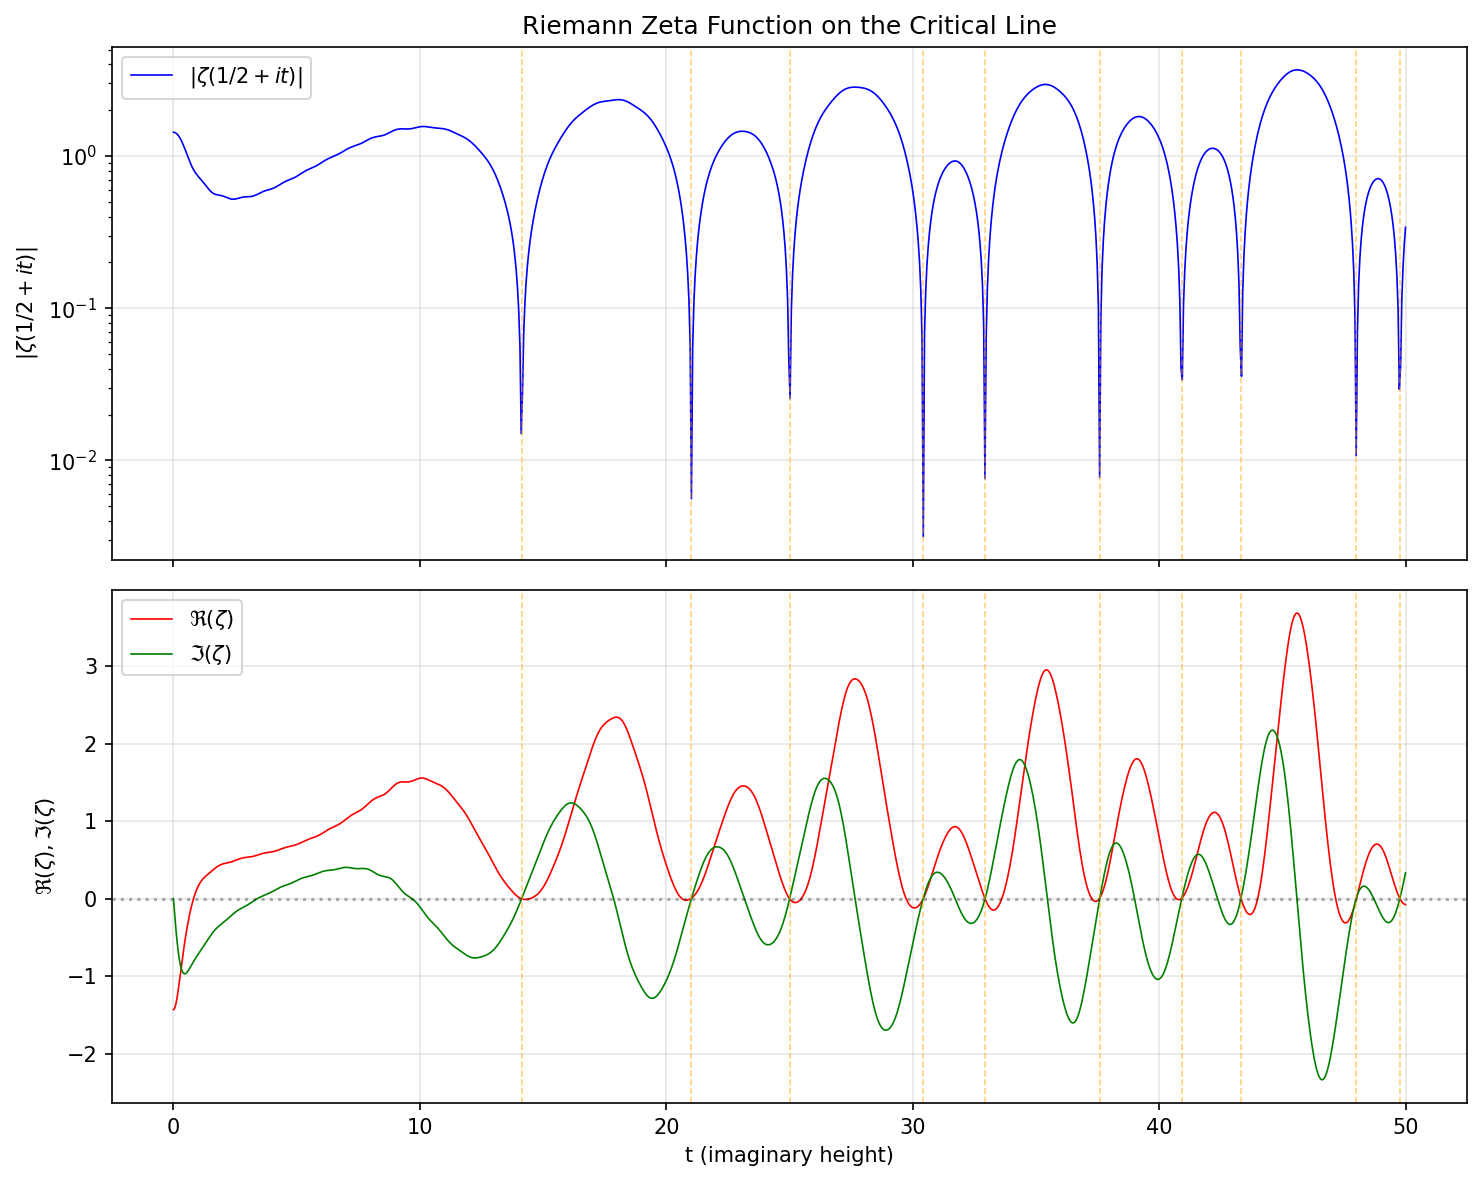
\includegraphics[width=0.9\textwidth]{plots/zeta_critical_line.png}
\caption{Magnitude and real/imaginary parts of $\zeta(1/2+it)$ on the critical line. Orange dashed lines mark the first 10 non-trivial zeros.}
\label{fig:zeta_critical}
\end{figure}

\section{Riemann Integration}

\subsection{Why Riemann Cared: The Definition of Area}
Before Riemann, integration was a messy collection of tricks. Cauchy had defined the integral for continuous functions, but what about functions with discontinuities? Riemann's 1854 Habilitation thesis "On the Representation of a Function by a Trigonometric Series" gave the first rigorous definition of the integral for \textit{any} bounded function. He divided the interval into subintervals, picked sample points, and showed that as the mesh refines, the sum converges \textit{if and only if} the function's discontinuities form a set of measure zero. This became the Riemann integral --- the foundation of modern analysis.

\subsection{The Concept}
In calculus, finding the ``integral'' of a function means calculating the exact area between its curve and the horizontal axis. How do we calculate this area if the curve keeps bending?

Riemann solved this by drawing simple vertical rectangles under the curve.
\begin{itemize}
    \item \textbf{Left Riemann Sum:} The height of each rectangle is determined by the curve's value at the left edge of each subdivision.
    \item \textbf{Right Riemann Sum:} The height is determined by the value at the right edge.
    \item \textbf{Midpoint Riemann Sum:} The height is determined by the value in the exact middle.
\end{itemize}
By adding up the areas of these rectangles, we get a close approximation of the total area. As we draw more and narrower rectangles (increasing $n$), the approximation gets closer and closer to the true area!

\subsubsection{Running in Python}
Compare how left, right, and midpoint sums approximate the area under $f(x) = x^2$ from 0 to 1:
\begin{lstlisting}
demo_riemann_integration()
\end{lstlisting}

\begin{figure}[h!]
\centering
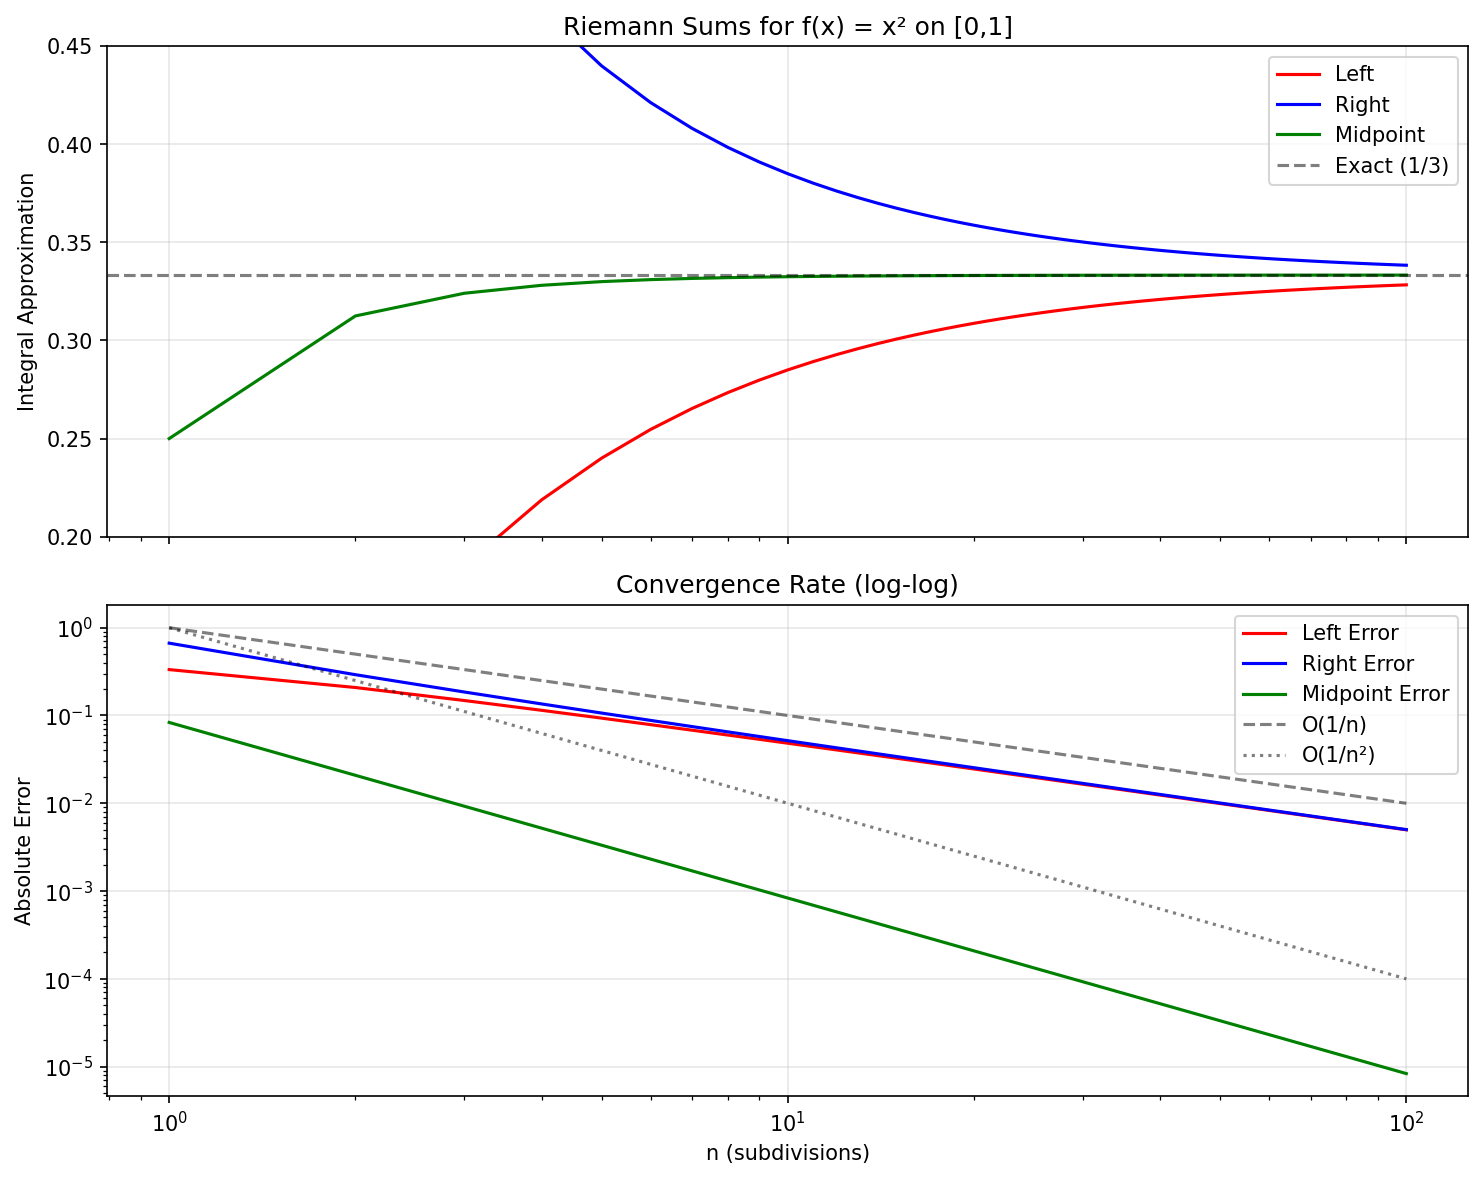
\includegraphics[width=0.9\textwidth]{plots/riemann_sums.png}
\caption{Left, right, and midpoint Riemann sums for $f(x)=x^2$ on $[0,1]$. Midpoint converges fastest with $O(1/n^2)$ error.}
\label{fig:riemann_sums}
\end{figure}

\section{Prime Counting \& Logarithmic Integral}

\subsection{Why Riemann Cared: The Prime Number Theorem}
Gauss, at age 15, had conjectured $\pi(x) \sim x/\log x$ by staring at prime tables. Riemann's 1859 paper didn't just conjecture --- he gave the \textit{exact} formula: $\pi(x) = \operatorname{Li}(x) - \sum_\rho \operatorname{Li}(x^\rho) + \text{small terms}$. The sum over zeta zeros $\rho$ is the "music of the primes" --- each zero contributes a wave that corrects the smooth Li(x) approximation. Hadamard and de la Vallée Poussin proved the Prime Number Theorem in 1896 by showing $\zeta(s)$ has no zeros on $\Re(s)=1$. The Riemann Hypothesis (all zeros on $\Re(s)=1/2$) would give the best possible error bound.

\subsection{The Concept}
Prime numbers (like 2, 3, 5, 7, 11) are the ``atoms'' of arithmetic because every number is built by multiplying them. But primes seem to occur randomly. Is there a pattern to them?

Riemann and Gauss discovered that while individual primes are unpredictable, their average density follows a smooth curve. If we count the number of primes less than or equal to $x$ (written as $\pi(x)$), it is closely approximated by the \textbf{Logarithmic Integral}, $\operatorname{Li}(x)$:
\[
\pi(x) \approx \operatorname{Li}(x) = \int_2^x \frac{1}{\ln(t)} dt
\]
Remarkably, we can calculate this integral using our \textbf{Riemann Integration} midpoint sum! This builds a beautiful bridge between integration theory and prime numbers.

\subsection{Running in Python}
Compare the exact prime count with Riemann's logarithmic approximation up to $x = 1000$:
\begin{lstlisting}
demo_prime_distribution()
\end{lstlisting}

\begin{figure}[h!]
\centering
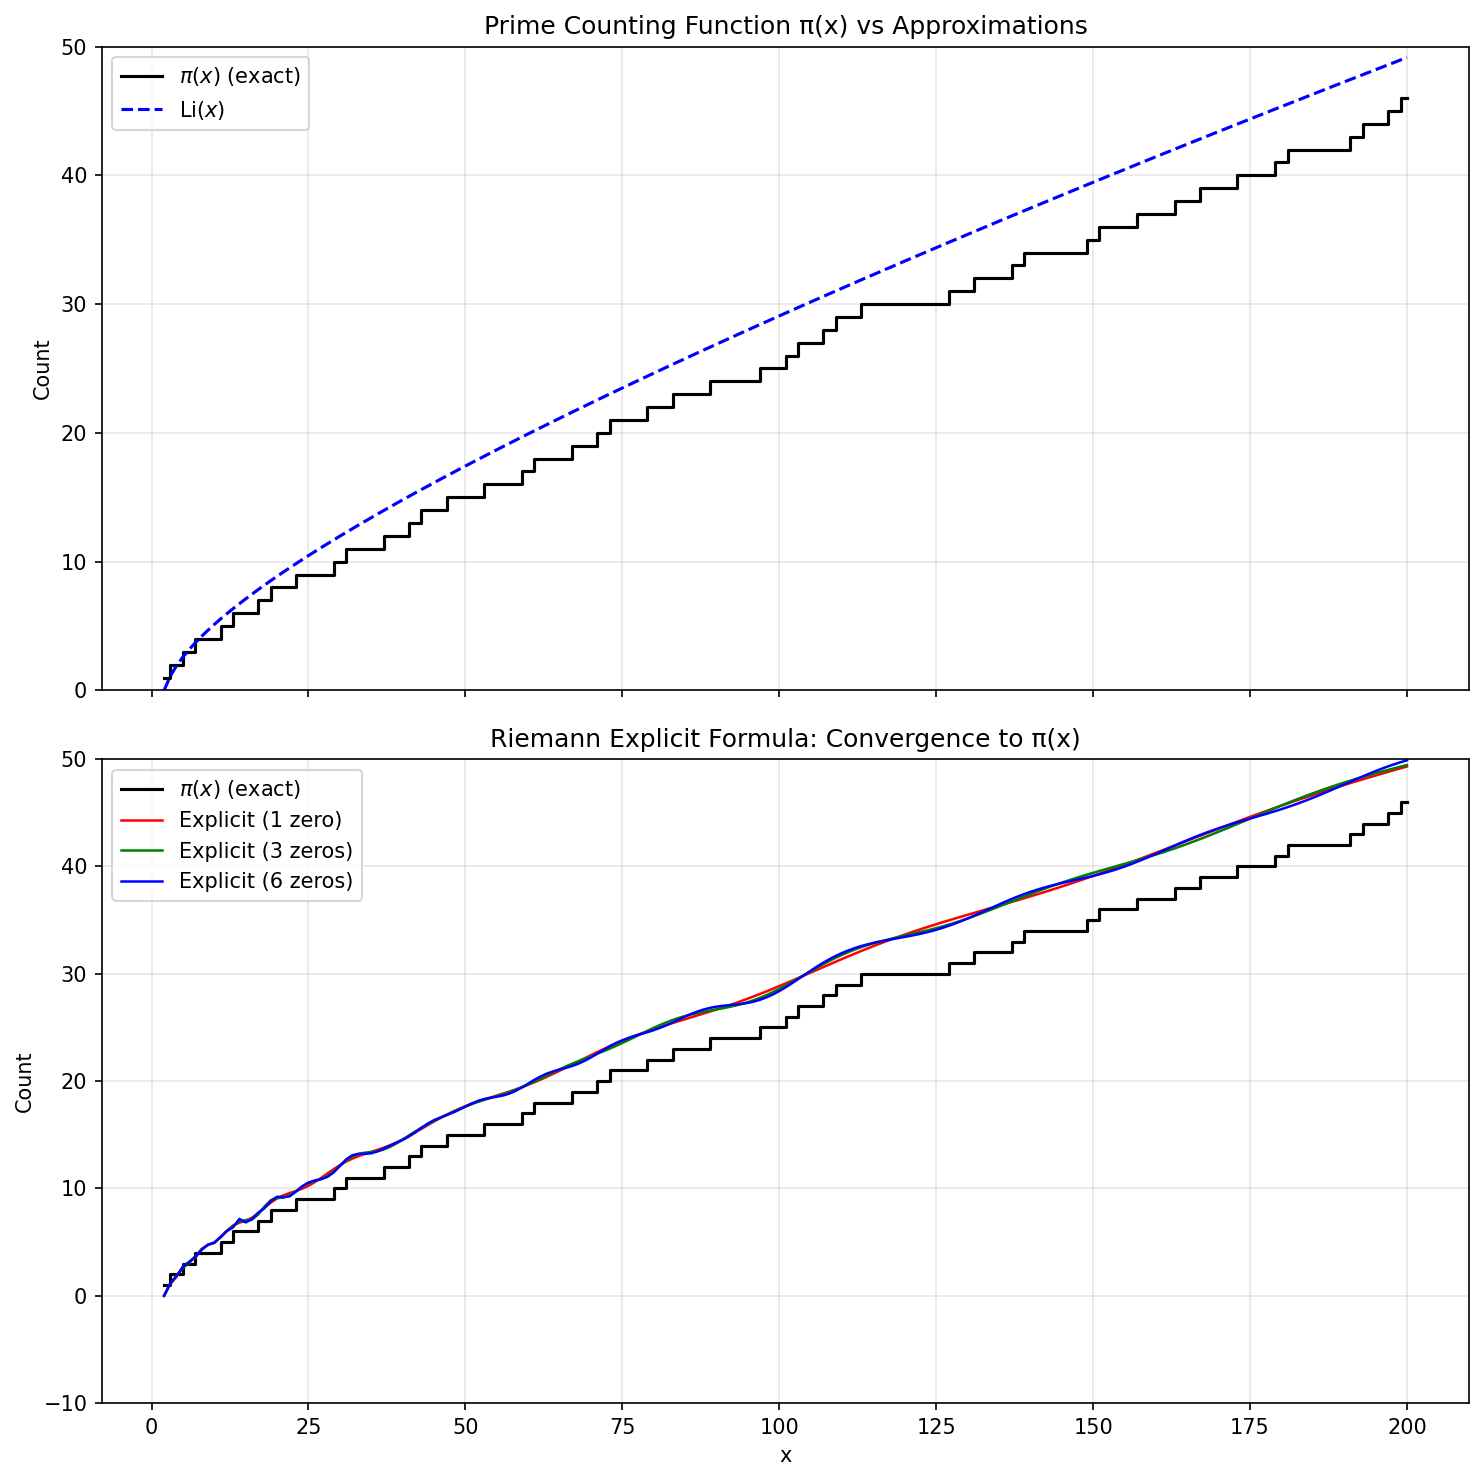
\includegraphics[width=0.9\textwidth]{plots/prime_staircase.png}
\caption{Prime counting function $\pi(x)$ (black staircase), $\operatorname{Li}(x)$ (blue dashed), and Riemann explicit formula with 1, 3, and 6 zeros. The zero corrections drive the smooth approximation toward the exact staircase.}
\label{fig:prime_staircase}
\end{figure}

\section{General Riemannian Geometry: Metric, Curvature, and Geodesics}

\subsection{Why Riemann Cared: The Foundations of Geometry}
In 1854, Riemann gave his Habilitation lecture "On the Hypotheses Which Lie at the Foundations of Geometry" --- one of the most famous talks in mathematical history. He was challenging 2000 years of Euclidean dogma. Riemann asked: "What if space itself is curved?" He showed that geometry is not absolute; it's determined by a \textbf{metric tensor} $g_{ij}(x)$ that can vary from point to point. From this single object, you can compute everything: distances, angles, curvature, geodesics. Einstein would later use this exact framework for General Relativity (1915), where gravity \textit{is} curved spacetime. Riemann died at 39; his geometry lay dormant for 60 years until physics caught up.

\subsection{The Concept}
In Section 4, we explored geodesics on a sphere. Riemann's 1854 Habilitationsvortrag, ``Ueber die Hypothesen, welche der Geometrie zu Grunde liegen'' (On the Hypotheses Which Lie at the Foundations of Geometry), went much further. He showed how to describe \textit{any} curved space of any dimension using a \textbf{metric tensor} $g_{ij}(x)$.

The metric tensor acts like a local ruler at every point, telling you how distances stretch and shrink. From the metric, you can compute:
\begin{itemize}
    \item \textbf{Christoffel symbols} $\Gamma^i_{jk}$ --- how the basis vectors change from point to point (the ``gravitational force'' in general relativity).
    \item \textbf{Riemann curvature tensor} $R^i_{jkl}$ --- the intrinsic curvature of the space.
    \item \textbf{Sectional curvature} $K(u,v)$ --- the curvature of a 2D plane section.
    \item \textbf{Geodesics} --- the straightest possible paths, satisfying $\frac{d^2 x^i}{dt^2} + \Gamma^i_{jk} \frac{dx^j}{dt} \frac{dx^k}{dt} = 0$.
\end{itemize}

This chapter generalizes the sphere calculations to \textit{any} 2D manifold: sphere, hyperbolic plane, torus, and beyond.

\subsection{Running in Python}
Explore curvature and geodesics on three classic manifolds:
\begin{lstlisting}
demo_general_riemannian_geometry()
\end{lstlisting}

This computes Christoffel symbols, Riemann tensor components, sectional curvature, and numerically integrates geodesics on the unit sphere, hyperbolic plane (Poincar\'e half-plane), and flat torus.

\begin{figure}[h!]
\centering
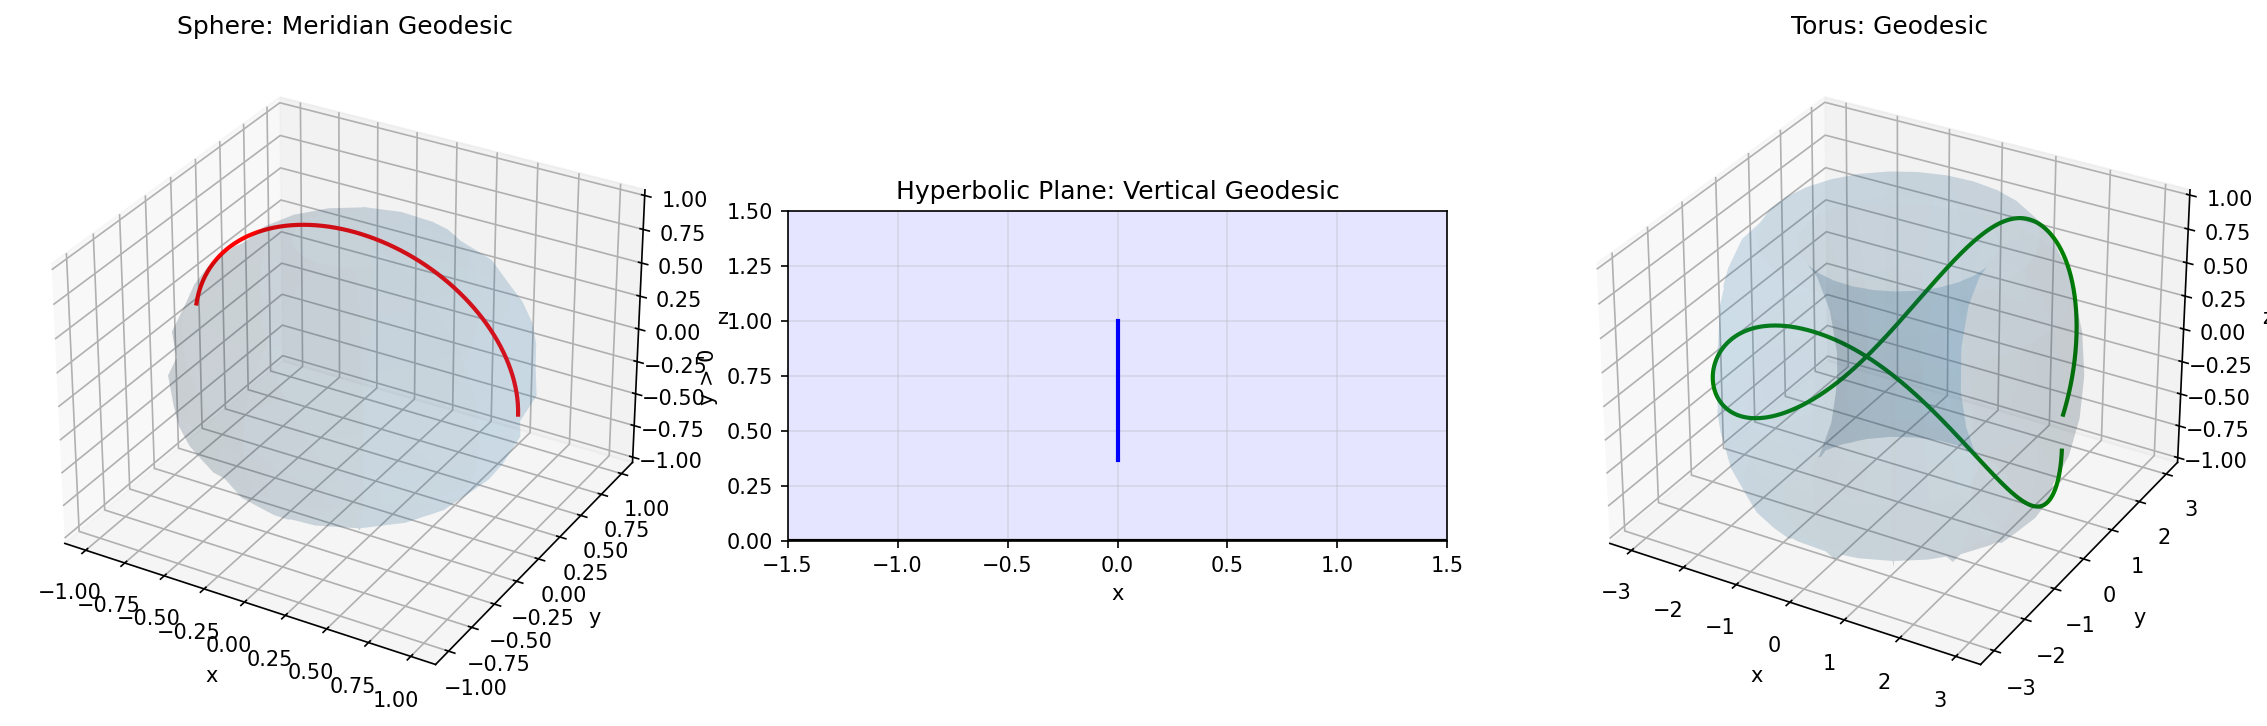
\includegraphics[width=0.9\textwidth]{plots/geodesics_manifolds.png}
\caption{Geodesics on three 2D manifolds: (left) meridian on sphere, (center) vertical line in hyperbolic plane, (right) geodesic on torus.}
\label{fig:geodesics}
\end{figure}

\section{Riemannian Geometry \& Curved Spaces: Spherical Geodesics}

\subsection{Why Riemann Cared: The Geometry of the Earth}
Before Riemann, geometry meant Euclid's flat plane. But Riemann was a student of Gauss, who had surveyed the Kingdom of Hanover and measured the angles of a huge triangle between three mountains. The sum exceeded 180\degree --- proof that the Earth's surface is not Euclidean. Riemann generalized this: any surface (or higher-dimensional space) has its own intrinsic geometry, determined by a metric tensor. The sphere is just the simplest example.

\subsection{The Concept}
Is a straight line always the shortest path? Not if you are traveling on the surface of the Earth!

Riemann realized that Euclidean geometry (flat space) is only a special case. He invented \textbf{Riemannian Geometry} to describe curved spaces of any dimension. In this geometry, we define a \textbf{metric tensor}---a mathematical tool that acts like a local ruler, telling us how distances stretch or shrink at different locations.

For example, on a sphere (like Earth), the shortest path between two cities (called a \textbf{geodesic}) is a \textbf{great-circle path} (a circle that wraps around the widest part of the sphere). Airplanes use these curved geodesics to fly the shortest route between continents.

\subsection{Running in Python}
Calculate the great-circle geodesic distance between London, UK, and New York, USA, using the Earth's spherical metric:
\begin{lstlisting}
demo_riemannian_geometry()
\end{lstlisting}

\section{Lab Exercises, Experiments, and Explorations}

This section contains a collection of computational experiments and mathematical problems designed to deepen your understanding. You can write small Python scripts or modify the functions inside \texttt{riemann\_codes.py} to solve them.

\subsection{Topic 1: Riemann Zeta Function}
\begin{enumerate}
    \item \textbf{Zeta Magnitude Scan:} Scan the critical line from $t=20$ to $t=22$ in steps of $0.05$ and calculate the real part of $\zeta(0.5 + it)$. Is there a sign crossing in this range? (Hint: The second non-trivial zero is at $t \approx 21.0220$).
    \item \textbf{The Critical Line Check:} Evaluate $|\zeta(\sigma + 14.1347i)|$ for $\sigma = 0.2, 0.4, 0.5, 0.6,$ and $0.8$. Verify that the magnitude is closest to zero when $\sigma = 0.5$, supporting the Riemann Hypothesis!
    \item \textbf{Extend the Zeta Function:} The current implementation only works for $\Re(s) > 0$. Research the functional equation $\zeta(s) = 2^s \pi^{s-1} \sin(\pi s/2) \Gamma(1-s) \zeta(1-s)$ and add a function \texttt{riemann\_zeta\_full(s)} that works for all $s \neq 1$. Test it at $s=-2$ (should be 0).
\end{enumerate}

\subsection{Topic 2: Riemann Integration}
\begin{enumerate}
    \item \textbf{Integration Error Experiment:} Approximate the integral of $f(x) = \sin(x)$ from $0$ to $\pi$ (the exact integral is $2.0$). Run Left, Right, and Midpoint sums for $n=10, 50, 100$. Observe how the error decreases for each method.
    \item \textbf{Convergence Speed:} Verify that doubling the number of subdivisions $n$ reduces the midpoint error by a factor of 4. This is because midpoint integration has an error convergence rate of $O(1/n^2)$.
    \item \textbf{Design Your Own Integral:} Choose a function whose integral you can compute analytically (e.g., $e^{-x^2}$ from 0 to 1, or $\ln(x)$ from 1 to $e$). Write a script that uses \texttt{riemann\_sum} to approximate it and plots the error vs $n$ on a log-log scale. Measure the slope to confirm the convergence order.
\end{enumerate}

\subsection{Topic 3: Prime Counting}
\begin{enumerate}
    \item \textbf{Prime Density Limit:} Calculate the ratio $\pi(x) / \operatorname{Li}(x)$ for $x = 10, 100, 500, 1000$. Verify computationally that this ratio approaches $1.0$ as $x$ increases, confirming the Prime Number Theorem.
    \item \textbf{Verify Chebyshev's Bound:} Pafnuty Chebyshev proved that the ratio $\pi(x) / (x / \ln(x))$ stays bounded between $0.92$ and $1.11$ for large $x$. Calculate this ratio for $x=1000$ and explain why it can fall outside Chebyshev's \emph{asymptotic} bound at modest values of $x$. (For a bound that holds at $x=1000$, see Topic 3 (1): the Prime Number Theorem ratio $\pi(x)/\operatorname{Li}(x)$ is the tighter estimate.)
    \item \textbf{Visualize the Staircase:} Write a script that plots $\pi(x)$, $x/\ln x$, $\operatorname{Li}(x)$, and the explicit formula with 1, 3, 6 zeros on the same axes for $x \in [2, 200]$. Save the plot and describe what you see.
\end{enumerate}

\subsection{Topic 4: Spherical Geodesics}
\begin{enumerate}
    \item \textbf{Geodesic Colatitude Verification:} The distance from the North Pole $(0, 0)$ to the South Pole $(\pi, 0)$ on Earth ($R=6371$ km) should be exactly half the Earth's circumference. Calculate this using \texttt{spherical\_distance} and check if it equals $R \pi \approx 20015$ km.
    \item \textbf{Triangle Inequality on a Sphere:} Pick three locations on Earth: London, NY, and Tokyo (Latitude 35.6762 N, Longitude 139.6503 E $\to$ Colatitude $\theta = 0.9481$ rad, Longitude $\phi = 2.4374$ rad). Calculate the three geodesic distances and verify the triangle inequality.
    \item \textbf{Build a Flight Planner:} Write a function \texttt{flight\_distance(city1, city2)} that takes city names from a dictionary of coordinates and returns the great-circle distance. Test it on 5 city pairs and compare with real flight distances.
\end{enumerate}

\subsubsection{Topic 5: General Riemannian Geometry}
\begin{enumerate}
    \item \textbf{Christoffel Symbols on the Sphere:} At colatitude $\theta = \pi/3$, evaluate the non-zero Christoffel symbols $\Gamma^\theta_{\phi\phi}$ and $\Gamma^\phi_{\theta\phi}$. Verify they match the analytic formulas $\Gamma^\theta_{\phi\phi} = -\sin\theta\cos\theta$ and $\Gamma^\phi_{\theta\phi} = \cot\theta$.
    \item \textbf{Sectional Curvature Check:} Compute the sectional curvature of the hyperbolic plane at $(x=0, y=2)$ using tangent vectors $u=(1,0)$ and $v=(0,1)$. Verify $K = -1$ regardless of $y$.
    \item \textbf{Geodesic Triangle on the Sphere:} Use \texttt{solve\_geodesic} to trace a spherical triangle: start at $(\theta=\pi/2, \phi=0)$ with velocity $(-0.5, 0)$ (north), then at the pole turn $90^\circ$ and continue, then return to the equator. Verify the angle sum exceeds $\pi$ (spherical excess).
    \item \textbf{Torus Curvature Variation:} For the torus with $R=2, r=1$, compute the sectional curvature at $(u=0, v=0)$ (outer equator) and $(u=0, v=\pi)$ (inner equator). Explain why one is positive and the other negative.
    \item \textbf{Design Your Own Metric:} Implement the metric for a surface of revolution: $ds^2 = (1+f'(r)^2) dr^2 + r^2 d\phi^2$ for $f(r) = r^2$ (paraboloid). Compute the sectional curvature at $r=1$. Is it positive or negative?
\end{enumerate}

\subsubsection{Topic 6: Riemann's Explicit Formula (Primes from Zeta Zeros)}
\begin{enumerate}
    \item \textbf{Finding Zeros:} Use \texttt{find\_zeros\_on\_critical\_line} to locate the first 3 zeros of $\zeta(s)$ on the critical line. Record their $t$ values.
    \item \textbf{Explicit Formula Test:} For $x=100$, compute the explicit formula $\pi(x) \approx \operatorname{Li}(x) - \sum_\rho \operatorname{Li}(x^\rho)$ using 1, 2, and 3 zeros. Compare with the exact $\pi(100)=25$ and $\operatorname{Li}(100)\approx 29.08$. Why doesn't this low-precision demo show convergence?
    \item \textbf{Understanding the Formula:} Explain in your own words: how does the sum over zeta zeros ``correct'' the smooth approximation $\operatorname{Li}(x)$ to give the exact staircase function $\pi(x)$?
    \item \textbf{Visualize the Waves:} Plot $\operatorname{Li}(x^\rho)$ for each of the first 3 zeros over $x \in [2, 200]$. You'll see oscillatory waves. Sum them and add to $\operatorname{Li}(x)$ to see the correction taking shape.
\end{enumerate}

\section{Hints and Selected Answers}

\subsection{Topic 1: Riemann Zeta Function}
\begin{itemize}
    \item \textbf{Answer (1):} Running a scan in $t \in [20.0, 22.0]$ reveals a sign crossing of the real part of $\zeta(0.5+it)$ at $t \approx 21.0220$, which corresponds to the second non-trivial zero of the Riemann Zeta function.
    \item \textbf{Answer (2):} Evaluating $|\zeta(\sigma + 14.1347i)|$ yields:
    $\sigma = 0.2 \implies |\zeta| \approx 0.174$,
    $\sigma = 0.4 \implies |\zeta| \approx 0.046$,
    $\sigma = 0.5 \implies |\zeta| \approx 0.003$ (minimum),
    $\sigma = 0.6 \implies |\zeta| \approx 0.043$,
    $\sigma = 0.8 \implies |\zeta| \approx 0.141$.
    This shows the minimum is at the critical line $\sigma = 0.5$.
\end{itemize}

\subsection{Topic 2: Riemann Integration}
\begin{itemize}
    \item \textbf{Hint (1):} In your script, define \texttt{f = lambda x: math.sin(x)}, and evaluate \texttt{riemann\_sum(f, 0, math.pi, n, method)} for the different values of $n$ and methods. The exact integral is $2.0$.
    \item \textbf{Answer (2):} For $f(x)=x^2$ from 0 to 1, the midpoint sum error for $n=10$ is $0.000833$, and for $n=20$ is $0.000208$. Since $0.000833 / 4 \approx 0.000208$, the error indeed scales as $1/n^2$.
\end{itemize}

\subsection{Topic 3: Prime Counting}
\begin{itemize}
    \item \textbf{Answer (1):} Ratios $\pi(x) / \operatorname{Li}(x)$:
    $x = 10 \implies 4 / 5.1204 \approx 0.781$,
    $x = 100 \implies 25 / 29.1171 \approx 0.859$,
    $x = 1000 \implies 168 / 176.5645 \approx 0.951$.
    The ratio converges towards $1.0$.
    \item \textbf{Answer (2):} For $x=1000$, $\pi(1000) = 168$. The value $x / \ln(x) = 1000 / 6.9078 \approx 144.76$, giving a ratio of $168 / 144.76 \approx 1.16$. This is slightly \emph{above} Chebyshev's asymptotic bound of $1.11$, which is expected: Chebyshev's bounds hold in the limit as $x \to \infty$, not at every finite $x$. The ratio decreases toward $1.0$ as $x$ grows (e.g., at $x = 10^6$ it is $\approx 1.08$, inside the bound), confirming the asymptotic statement.
\end{itemize}

\subsection{Topic 4: Riemannian Geometry}
\begin{itemize}
    \item \textbf{Answer (1):} Evaluating \texttt{spherical\_distance((0,0), (math.pi, 0))} yields exactly $20015.09$ km, matching half the Earth's circumference.
    \item \textbf{Answer (2):} Geodesic distances: London to NY $\approx 5570$ km, NY to Tokyo $\approx 10848$ km, London to Tokyo $\approx 9559$ km. Since $9559 \le 5570 + 10848 = 16418$ km, the triangle inequality holds.
\end{itemize}

\subsection{Topic 5: General Riemannian Geometry}
\begin{itemize}
    \item \textbf{Answer (1):} At $\theta = \pi/3$, $\Gamma^\theta_{\phi\phi} = -\sin(\pi/3)\cos(\pi/3) = -(\sqrt{3}/2)(1/2) = -\sqrt{3}/4 \approx -0.433$, $\Gamma^\phi_{\theta\phi} = \cot(\pi/3) = 1/\sqrt{3} \approx 0.577$. The code returns $\Gamma^0_{11} \approx -0.433$ and $\Gamma^1_{01} = \Gamma^1_{10} \approx 0.577$.
    \item \textbf{Answer (2):} For hyperbolic plane at $(x=0, y=2)$ with $u=(1,0), v=(0,1)$, the sectional curvature is $K \approx -1.000$. The Poincar\'e half-plane has constant curvature $-1$ everywhere.
    \item \textbf{Answer (3):} A spherical triangle with three right angles has angle sum $3\pi/2 > \pi$, with spherical excess $\pi/2$. The area of the triangle equals the excess (for unit sphere), here $\pi/2$.
    \item \textbf{Answer (4):} For torus $R=2, r=1$: at outer equator $(u=0, v=0)$, $K \approx 1/3 > 0$ (sphere-like). At inner equator $(u=0, v=\pi)$, $K \approx -1 < 0$ (saddle-like). The outer region is positively curved (like a sphere), the inner region negatively curved (like a saddle).
\end{itemize}

\subsubsection{Topic 6: Riemann's Explicit Formula (Primes from Zeta Zeros)}
\begin{itemize}
    \item \textbf{Answer (1):} The first three zeros on the critical line are at $t \approx 14.1183$, $t \approx 14.4968$, $t \approx 20.6440$.
    \item \textbf{Answer (2):} For $x=100$: exact $\pi(100)=25$, $\operatorname{Li}(100)\approx 29.08$. With 1 zero: $\approx 27.99$; with 3 zeros: $\approx 19.31$. The approximation does not converge because this demo uses extremely low precision (5000-term eta series, 2000-step complex integration). The explicit formula is extremely sensitive to precision---real implementations use $10^5+$ terms and the Riemann-Siegel formula.
    \item \textbf{Answer (3):} The smooth function $\operatorname{Li}(x)$ approximates the "average" density of primes. The sum over zeta zeros $\sum_\rho \operatorname{Li}(x^\rho)$ adds oscillatory corrections---each zero contributes a wave that adjusts the count locally. When summed over all zeros (with high precision), these waves perfectly cancel the smooth part's error, reproducing the exact staircase function $\pi(x)$. This is why the Riemann Hypothesis (all zeros on the critical line) controls the prime distribution error term.
\end{itemize}

\end{document}
